% ======================================================
% Compile: xelatex 5state_aprime_axm_num.tex
% Path:    reference/eq17_analysis/derivation/5state_aprime_axm_num.tex
% DRAFT (2026-07-21, Windows). MEASUREMENT-NUMERATOR variant of the co-update:
% the var-ratio numerator is built from the a_xm MEASUREMENT (not the estimate
% a_hat), so the self-copy (kappa=0) is broken by construction (kappa=1). Anchor
% lag is pre-compensated in closed form; the a_xm noise floor R2 is subtracted
% explicitly; the denominator is the delay-aligned dh1. Template/route mirror
% 5state_aprime_coupdate.tex: 0 Def / 1 True / 2 a'_hdm / 3 Esti (co-update) /
% 4 Error / 5 F_e,H / 6 Q,R / 7 Regression (noise-linear limit) / 8 Simulation /
% 9 Verdict.
% ======================================================
\documentclass[11pt,a4paper,fontset=none]{ctexart}

\usepackage[fleqn]{amsmath}
\usepackage{amssymb,bm}
\usepackage{empheq}
\setlength{\mathindent}{0pt}
\usepackage{geometry}
\geometry{margin=2.1cm}
\usepackage{array,booktabs}
\usepackage{graphicx}
\usepackage{xcolor}

\setlength{\parindent}{0pt}
\setlength{\parskip}{1.35em}
\setlength{\abovedisplayskip}{17pt}
\setlength{\belowdisplayskip}{17pt}
\setlength{\abovedisplayshortskip}{11pt}
\setlength{\belowdisplayshortskip}{11pt}
\linespread{1.08}\selectfont

\newcommand{\lc}{\lambda_c}
\newcommand{\ap}{a'_{hd}}
\newcommand{\aph}{\hat a'_{hd}}
\newcommand{\apm}{a'_{hdm}}
\newcommand{\apmh}{\hat a'_{hdm}}
\newcommand{\dxh}{\delta\hat h}
\newcommand{\ghp}{g_{\mathrm{hp}}}
\newcommand{\Rint}{R_2^{\mathrm{int}}}
\newcommand{\hd}[2]{\par\bigskip\noindent%
  \underline{\textbf{#1}}\quad{\small\itshape #2}\par\nobreak\vspace{0.9ex}}

\begin{document}

% ------------------------------------------------------------------
\hd{0. Definitions}{coordinates, slope $\ap$, tracking error, gain measurement $a_{xm}$}

\[
h[k] = h_d[k] - \delta h[k], \qquad
\Delta h_d[k] = h_d[k+1] - h_d[k], \qquad
\delta h_1 := \delta h[k-d],\ \ d=2
\]
\[
\ap[k] := \left.\frac{d a_h}{d h}\right|_{h_d[k]}, \qquad
a_r[k] := a_h[k] - a_h\big(h_d[k]\big)
\]
\[
\delta h[k+1] = \lc\,\delta h[k] - F_{dh}[k]\,e_{a_h}[k] - \varepsilon_h[k]
\]
\[
a_{xm}[k] = a_h[k-d] + n_a[k], \qquad
\mathrm{Var}(n_a) = \Rint, \qquad
\ghp := \frac{1-a_{var}}{a_{var}}, \qquad
\beta = 1-\frac{T_s}{\tau}
\]

% ------------------------------------------------------------------
\hd{1. True}{residual $=-\ap\,\delta h$; the measurement carries it delayed; the $\beta$-EWMA is the slope law}

\[
a_h\big(h[k]\big) \approx a_h\big(h_d[k]\big) - \ap[k]\,\delta h[k]
\]
\begin{empheq}[box=\fbox]{equation*}
a_r[k] = -\,\ap[k]\,\delta h[k], \qquad \ap[k+1]\approx\ap[k]
\end{empheq}
\[
\apm[k] := +\sqrt{\;\mathrm{Var}\big(a_r[k]\big)\,/\,\mathrm{Var}\big(\delta h[k]\big)\;}
= \ap[k] \qquad(\ap>0)
\]
\[
A[k] := a_h\big(h_d[k-d]\big), \qquad
a_{xm}[k] = A[k] - \ap\,\delta h_1[k] + n_a[k]
\]
\begin{empheq}[box=\fbox]{equation*}
\ap[k+1] = \beta\,\ap[k] + (1-\beta)\,\apm[k], \qquad \apm \equiv \ap
\end{empheq}

% ------------------------------------------------------------------
\hd{2. $\apmh$}{measurement numerator: anchor-lag pre-compensation, floor subtraction, delay-aligned denominator}

\[
\begin{aligned}
\overline a_{xm}[k+1] &= (1-a_{var})\,\overline a_{xm}[k] + a_{var}\,a_{xm}[k+1],
  & a_{xm,r}[k] &= a_{xm}[k] - \overline a_{xm}[k] \\[2pt]
\overline{\dxh_1}[k+1] &= (1-a_{var})\,\overline{\dxh_1}[k] + a_{var}\,\dxh_1[k+1],
  & \dxh_{1,r}[k] &= \dxh_1[k] - \overline{\dxh_1}[k]
\end{aligned}
\]
\[
a_{xm,r}[k] = \mathrm{HP}[A][k] \;-\; \ap\,\delta h_1[k] \;+\; n_a[k]
\]
\begin{empheq}[box=\fbox]{equation*}
\mathrm{HP}[A][k] \approx \ghp\,\frac{dA}{dk} = \ghp\,\ap[k]\,\Delta h_d[k]
\end{empheq}
\begin{empheq}[box=\fbox]{equation*}
a_{xm,r}^{\mathrm{corr}}[k]
= a_{xm,r}[k] - \ghp\,\aph[k]\,\Delta h_d[k]
= \ghp\,e_{\ap}[k]\,\Delta h_d[k] \;-\; \ap\,\delta h_1[k] \;+\; n_a[k]
\end{empheq}
\[
\hat\sigma^2_{a_{xm,r}}[k+1]
= (1-a_{cov})\,\hat\sigma^2_{a_{xm,r}}[k] + a_{cov}\,\big(a_{xm,r}^{\mathrm{corr}}[k+1]\big)^2,
\qquad
\hat\sigma^2_{\dxh_1}[k+1]
= (1-a_{cov})\,\hat\sigma^2_{\dxh_1}[k] + a_{cov}\,\dxh_{1,r}^2[k+1]
\]
\begin{empheq}[box=\fbox]{equation*}
\apmh[k] := +\sqrt{\;
\big(\hat\sigma^2_{a_{xm,r}}[k] - \Rint[k]\big)^{+}\,\big/\,
\hat\sigma^2_{\dxh_1}[k]\;}
\end{empheq}
\[
e_{\ap}=0 \;\Rightarrow\;
\hat\sigma^2_{a_{xm,r}}-\Rint = \ap{}^2\,\sigma^2_{\delta h}
\;\Rightarrow\;
\apmh = \ap/\sqrt{\zeta} \approx \ap,
\qquad \zeta := \mathrm{Var}(\dxh_1)/\mathrm{Var}(\delta h) \approx 1
\]

% ------------------------------------------------------------------
\hd{3. Esti (co-update)}{$\ap$ is driven by the $\beta$-EWMA of $\apmh$ \emph{plus} the KF innovation correction}

\[
x = [\,\delta h_1,\ \delta h_2,\ \delta h_3,\ a_h,\ \ap\,]^{\mathsf T},
\qquad
K = P^-H^{\mathsf T}S^{-1},\quad S=HP^-H^{\mathsf T}+R
\]
\[
\hat a_h[k+1] = \hat a_h[k] + \aph[k]\big(\Delta h_d[k] + (1-\lc)\,\dxh_3[k]\big)
\]
\begin{empheq}[box=\fbox]{equation*}
\aph[k+1] =
\underbrace{\beta\,\aph[k] + (1-\beta)\,\apmh[k]}_{\text{var-ratio }\beta\text{-EWMA}}
\;+\;
\underbrace{L_{51}[k]\,e_{y_1}[k] + L_{52}[k]\,e_{y_2}[k]}_{\text{KF }L\cdot e}
\end{empheq}
\[
L_{5j}=[P^-H^{\mathsf T}S^{-1}]_{5,j} \;\propto\; P^-_{5,4}\ \ (\text{cross-cov, since }H(\cdot,5)=0),
\qquad P^-_{5,4}\ \text{built only by}\ F_e(4,5)=\Delta h_d
\]

% ------------------------------------------------------------------
\hd{4. Error}{$\kappa=1$: the readout carries a genuine error, not the $\hat a_h$ echo ($\kappa=0$)}

\[
e_{a_h}=a_h-\hat a_h, \quad e_{\ap}=\ap-\aph, \quad e_h=\delta h-\dxh
\]
\[
e_{a_h}[k+1] = \big(1+\aph F_{dh}\big)\,e_{a_h}
+ \Delta h_d\,e_{\ap} + (1-\lc)\,\aph\,e_h + \aph\,\varepsilon_h
\]
\begin{empheq}[box=\fbox]{equation*}
e_{\ap}[k+1] = \beta\,e_{\ap}[k]
\;-\;(1-\beta)\big(\apmh[k]-\apm[k]\big)
\;-\;(\text{KF correction}),
\qquad
\apmh-\apm = (\kappa{=}1)\ \text{error}+n_{var}
\end{empheq}

% ------------------------------------------------------------------
\hd{5. $\mathbf F_e$ and $\mathbf H$}{$F_e(4,5)=\Delta h_d$ is the only path giving $\ap$ a Kalman gain}

\[
F_e[k] =
\begin{bmatrix}
0 & 1 & 0 & 0 & 0 \\[2pt]
0 & 0 & 1 & 0 & 0 \\[2pt]
0 & 0 & \lc & -F_{dh}[k] & 0 \\[2pt]
0 & 0 & (1-\lc)\aph[k] & 1+\aph[k]F_{dh}[k] & \Delta h_d[k] \\[2pt]
0 & 0 & 0 & 0 & \beta
\end{bmatrix},
\qquad
H =
\begin{bmatrix}
1 & 0 & 0 & 0 & 0 \\[2pt]
0 & 0 & 0 & 1 & 0
\end{bmatrix}
\]

% ------------------------------------------------------------------
\hd{6. $\mathbf Q$ and $\mathbf R$}{variance-ratio readout noise is \emph{quadratic} in the floor}

\[
Q = \mathrm{diag}\big(0,\ 0,\ Q_{33},\ Q_{44},\ Q_{55}\big),
\qquad
R = \mathrm{diag}\big(\sigma^2_{n},\ \Rint\big),
\qquad
Q_{55}=(1-\beta)^2 R_{var}
\]
\[
Q_{33} = 4k_BT\,\hat a_h\big(1+(1-\lc)^2 d\big) + (1-\lc)^2\sigma^2_{n},
\qquad
Q_{44} = \big(\hat a_h K_h/R\big)^2\,\sigma^2_{\delta h},
\qquad
\Rint = a_{cov}\,IF_{var}\,\big(\hat a_h+\xi\big)^2
\]
\begin{empheq}[box=\fbox]{equation*}
R_{var} \;\approx\; \frac{a_{cov}\,IF}{4}\;
\frac{\big(\Rint\big)^{2}}{\ap{}^{2}\,\sigma^{4}_{\delta h}}
\qquad\text{(noise \emph{squared})}
\end{empheq}
\[
\text{colored-}a_{xm}:\ \ a_{xm}\ \text{is an IIR-variance output (slow)}\ \Rightarrow\
\text{its high-pass keeps only a fraction of }\Rint\ \Rightarrow\
\text{full-}\Rint\ \text{subtraction clamps }\sigma^2_{\mathrm{num}}\to0.
\]

% ------------------------------------------------------------------
\hd{7. Regression (noise-linear limit)}{optimizing the compensation over $\aph$ drops the floor from quadratic to linear}

\[
\aph{}^{\mathrm{reg}}[k] = \frac{\mathrm{Cov}\big(a_{xm,r},\,\Delta h_d\big)}
{\ghp\,\mathrm{Var}\big(\Delta h_d\big)},
\qquad
\mathrm{Cov}\big(a_{xm,r},\Delta h_d\big)
= \ghp\,\ap\,\mathrm{Var}(\Delta h_d)
\underbrace{+\,0}_{-\ap\delta h_1}
\underbrace{+\,0}_{n_a}
\]
\begin{empheq}[box=\fbox]{equation*}
\aph{}^{\mathrm{reg}} = \ap,
\qquad
R_{var}^{\mathrm{reg}} \;\approx\;
\frac{\Rint}{N_{\mathrm{eff}}\;\ghp^{2}\,\mathrm{Var}(\Delta h_d)}
\qquad\text{(noise \emph{linear})}
\end{empheq}
\[
R_{var}^{\mathrm{reg}}\propto \Rint \ \text{vs}\ R_{var}\propto(\Rint)^2;
\qquad
\text{but drive }\ghp\ap\Delta h_d \ll n_a,\ \ \text{and}\ \ \Delta h_d\!\to\!0\ \text{twice/cycle}.
\]

% ------------------------------------------------------------------
\hd{8. Simulation}{open-loop readout: the numerator cannot read $\ap$}

\begin{center}
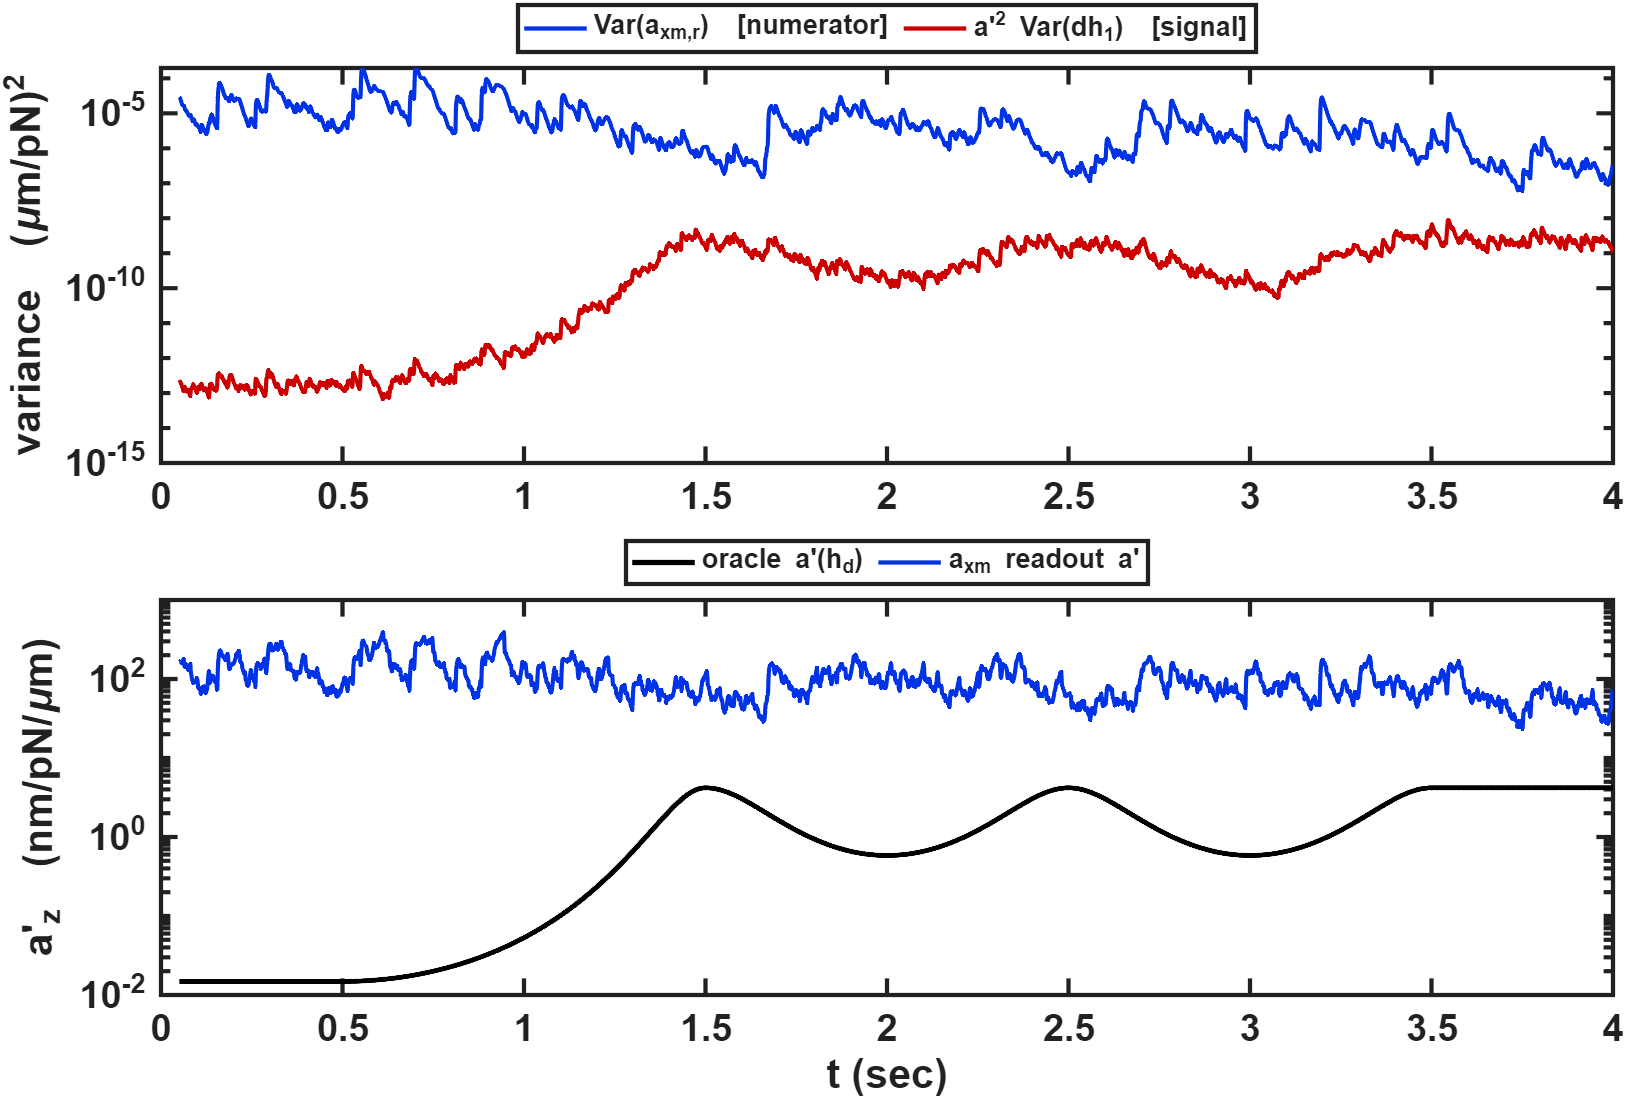
\includegraphics[width=0.92\textwidth]{figures/axm_num_varratio.png}
\end{center}
\textit{Open-loop $a_{xm}$ numerator (taylor 4-state, seed 1). Top: the numerator
variance $\mathrm{Var}(a_{xm,r})$ (blue) sits $\sim\!5\times10^{3}$ above the thermal
signal $\ap{}^2\mathrm{Var}(\delta h)$ (red) it should equal --- the $a_{xm}$ noise
floor. Bottom: the readout $\apmh=\sqrt{\,\cdot\,}$ is therefore $\sim\!70\times$
oracle $\ap(h_d)$ (black).}

% ------------------------------------------------------------------
\hd{9. Verdict}{$\kappa=1$, truth is a fixed point --- but the channel is below its own resolution}

\begin{empheq}[box=\fbox]{equation*}
\apmh/\ap \approx 70, \qquad
\big(\apmh/\ap\big)^2 = \frac{\mathrm{Var}(a_{xm,r})}{\ap{}^2\,\sigma^2_{\delta h}}
\approx 5\times10^{3}
\quad(\text{osc, near wall})
\end{empheq}

\[
\text{Structurally sound}\ (\kappa=1,\ \text{fixed point at }\ap,\ \text{no }c(\bar h))
\ \text{but information-limited: the readout is buried in the }a_{xm}\ \text{floor}.
\]
\[
\text{Past the floor}\ \Rightarrow\ \text{more information: trajectory dither}\
(\Delta h_d\ \text{non-zero-crossing})\ \text{or an independent }c\text{-free channel}.
\]

\end{document}
